\documentclass{beamer}
\usetheme{Madrid}
\usepackage[utf8]{inputenc}
\usepackage[ruled,linesnumbered]{algorithm2e}
\usepackage{amsmath,amsthm,amssymb,amsfonts}
\usepackage{mathtools}
\usepackage{booktabs}       % professional-quality tables
\usepackage{graphicx}
\usepackage{array}
\DeclareMathOperator*{\argmin}{argmin}
\DeclareMathOperator*{\argmax}{argmax}

\title[]{Empirical Analysis of Continuous Markov Data}
\subtitle{TTIC 31150 - Robotics}
\author[Lam, Sawhney, Yoo]{A. Lam \and K. Sawhney \and J. Yoo}

\date[June 2019]{June 2019}

\begin{document}

\frame{\titlepage}

\begin{frame}
\frametitle{Outline}
    \begin{enumerate}[I]
        \item Introduction
        \item HMM \& HSMM
        \item Data Generation
        \item Empirical Test
        \item Conclusion
    \end{enumerate}
\end{frame}


\begin{frame}
\frametitle{Introduction}
    \begin{itemize}
        \item Markov Model covered in class
        \begin{itemize}
            \item Abide by the markov assumption that state $X_{t+1}$ is conditioned on state $X_t$
            \item Discrete data (Integers) that represents colors or specific categories
        \end{itemize}
        \item Extension to the Markov Model
        \begin{itemize}
            \item Continuous data which observations are random variables (temperature, humidity, etc)
            \item Stickiness : Violation of markov assumption - probability of staying in the same state increases/decreases with each stay in the current state
        \end{itemize}
    \end{itemize}
\end{frame}

\begin{frame}
    \frametitle{Introduction}
        \begin{itemize}
            \item Research Question
            \begin{itemize}
                \item What is the best approach to do inference when data is continuous and markov assumption is violated? (HMM and HSMM)
                \item Does the setting of the maps have impact on the performance of these algorithms?
            \end{itemize}
        \end{itemize}
    \end{frame}

\begin{frame}
    \frametitle{HMM \& HSMM}
        \begin{itemize}
            \item HMM
        \end{itemize}
\end{frame}

\begin{frame}
    \frametitle{HMM \& HSMM}
        \begin{itemize}
            \item HSMM
        \end{itemize}
\end{frame}

\begin{frame}
    \frametitle{Data Generation}
        \begin{itemize}
            \item Gridworld setting
            \begin{itemize}
                \item Size : 5x5
                \item States : The observation at each states are Gaussian as $\mu$ as the true identity, $\sigma$ is universal across all states
                \item Obstacles : Different formation of obstacles indicate states that cannot be visited by the robot
            \end{itemize}
        \end{itemize}
\end{frame}

\begin{frame}
    \frametitle{Data Generation}
    \begin{itemize}
        \item Examples of map generation
    \end{itemize}
        \newcommand{\addmapa}{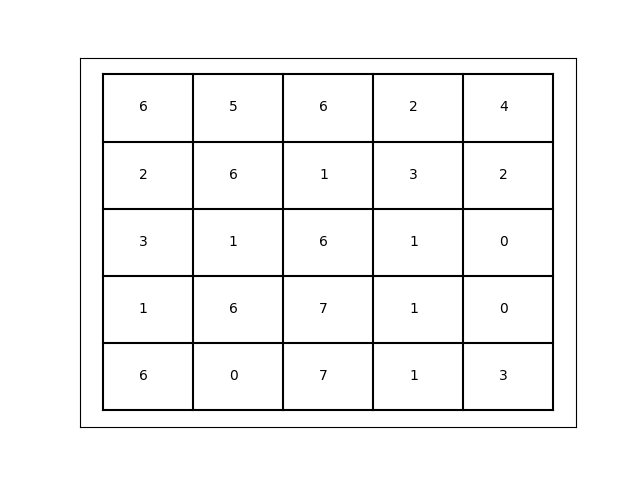
\includegraphics[width=10em]{data/Model1/5x5;4;free.png}}
        \newcommand{\addmapb}{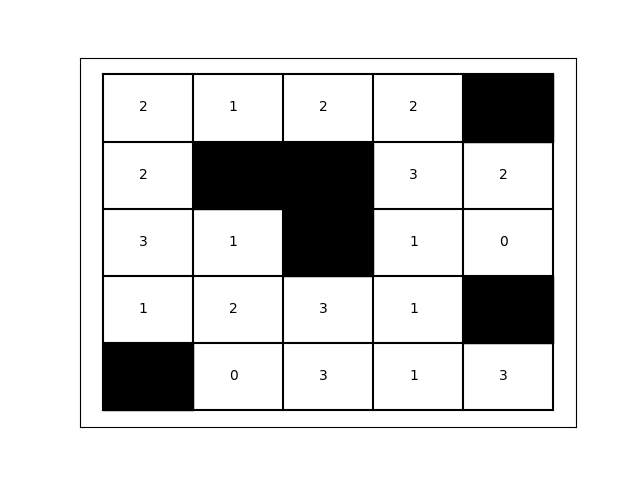
\includegraphics[width=10em]{data/Model2/5x5;4;6box.png}}
        \newcommand{\addmapc}{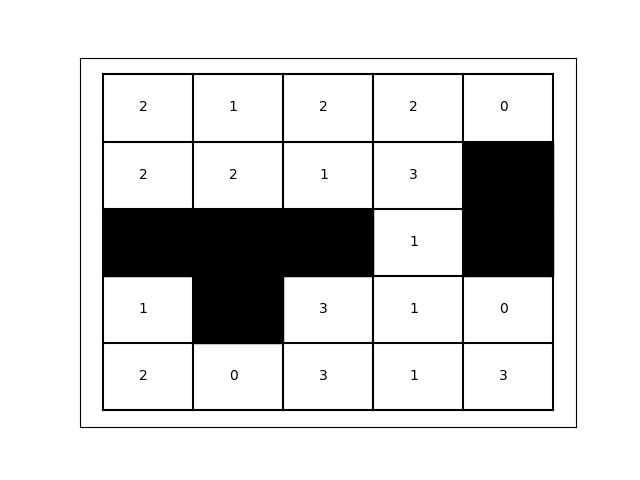
\includegraphics[width=10em]{data/Model3/5x5;4;6sep.png}}
        \newcolumntype{C}{>{\centering\arraybackslash}m{8em}}
        \begin{table}[H]
        \sffamily
        \centering
        \begin{tabular}{l*3{C}@{}}
        & \addmapa & \addmapb & \addmapc \\
        \end{tabular}
        \caption{GridWorld Maps}
        \end{table}
\end{frame}

\begin{frame}
    \frametitle{Emprical Results}
    \begin{itemize}
        \item Results
    \end{itemize}
\end{frame}


\begin{frame}
    \frametitle{References}
    \begin{itemize}
        \item [1] Johnson, M.J.\ \& Willsky, A.S.\ (2013) Bayesian Nonparametric Hidden Semi-Markov Models, {\it Journal of Machine Learning Research 14 (2013)},
        pp.\ 673--701. Cambridge, MA: MIT Press.
    \end{itemize}
\end{frame}

\end{document}
